\documentclass[12pt]{book} % Change to book
\usepackage{amsmath} % for mathematical expressions
\usepackage{xcolor} % for colored text
\usepackage{graphicx} % for including images
\usepackage{url}
\usepackage{booktabs} % for better-looking tables
\usepackage{makecell}
\usepackage{indentfirst}
\usepackage{algorithm}
\usepackage{algpseudocode}
\usepackage{amssymb}
\usepackage{placeins} % For \FloatBarrier
\usepackage{listings}
% Define the language style for Python code
\lstset{
    language=Python,
    basicstyle=\ttfamily,
    keywordstyle=\color{blue},
    stringstyle=\color{red},
    commentstyle=\color{gray},
    morecomment=[l][\color{magenta}]{\#},
    frame=single,
    breaklines=true
}
\begin{document}
\chapter{Approximation Algorithms}

\section{Introduction to Approximation Algorithms}

Approximation algorithms play a crucial role in tackling optimization problems where finding an exact solution is computationally infeasible. This section provides an overview of approximation algorithms, their definition, importance, role in solving NP-hard problems, and methods for evaluating their performance.

\subsection{Definition and Importance}

An \textbf{approximation algorithm} is an algorithm that finds a solution to an optimization problem that is guaranteed to be within a certain factor of the optimal solution. More formally, let \(A\) be an approximation algorithm for an optimization problem \(P\), and let \(OPT\) be the value of the optimal solution. \(A\) is called an \(\alpha\)-approximation algorithm if it always produces a solution with value at most \(\alpha \times OPT\), where \(\alpha\) is a constant greater than or equal to 1. In other words:

\[
\text{For maximization problems:} \quad A \geq \frac{1}{\alpha} \times OPT
\]
\[
\text{For minimization problems:} \quad A \leq \alpha \times OPT
\]

The approximation ratio \(\alpha\) quantifies the quality of the approximation obtained by the algorithm. A smaller value of \(\alpha\) indicates a better approximation.

Approximation algorithms are essential in practical settings where finding an exact solution is too time-consuming or even impossible. They provide solutions that are close to optimal and can be computed efficiently. These algorithms are widely used in various fields such as computer science, operations research, economics, and engineering for solving NP-hard and other optimization problems.

The importance of approximation algorithms can be observed in their ability to address real-world optimization problems effectively. For example, in scheduling problems, where finding an optimal schedule is NP-hard, approximation algorithms can provide near-optimal solutions within reasonable time frames, enabling efficient resource allocation and task scheduling in practice.

\subsection{Role of Approximation Algorithms in Solving NP-Hard Problems}

Approximation algorithms play a crucial role in tackling NP-hard problems, which are optimization problems for which no polynomial-time algorithm exists to compute an optimal solution, assuming $\text{P} \neq \text{NP}$. A classic example of the role of approximation algorithms in solving NP-hard problems is the \textbf{Vertex Cover} problem.


\subsubsection{Vertex Cover Problem}

Given an undirected graph \(G = (V, E)\), a \textbf{vertex cover} is a subset of vertices \(V'\) such that each edge in \(E\) is incident to at least one vertex in \(V'\). The goal is to find the smallest vertex cover in \(G\).

\paragraph{Approximation Algorithm: Greedy Vertex Cover}

A simple approximation algorithm for the Vertex Cover problem is the \textbf{Greedy Vertex Cover} algorithm:

\begin{algorithm}
\caption{Greedy Vertex Cover Algorithm}
\begin{algorithmic}[1]
\State $C \gets \emptyset$ \Comment{Initialize an empty vertex cover}
\While{there exists an uncovered edge $e = (u, v)$}
\State Add both $u$ and $v$ to $C$
\EndWhile
\State \textbf{return} $C$
\end{algorithmic}
\end{algorithm}

\paragraph{Example}

Consider the following graph \(G\):

\FloatBarrier
\begin{figure}[h]
    \centering
    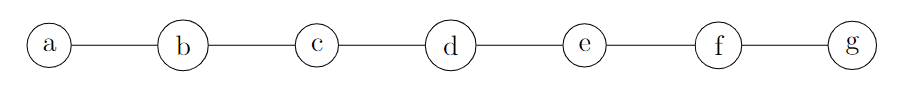
\includegraphics[width=0.6\textwidth]{images/Greedy_Vertex_Cover_Algorithm.png}
    \caption{Greedy Vertex Cover Algorithm}
\end{figure}
\FloatBarrier

The Greedy Vertex Cover algorithm will select vertices \(b\), \(d\), and \(f\) as the vertex cover, resulting in an approximation ratio of \(3\), as it selects three vertices while the optimal solution requires only one vertex.

\subsection{Evaluating Approximation Algorithms}

The performance of approximation algorithms is evaluated based on several criteria, including approximation ratio, running time, and worst-case analysis.

\subsubsection{Approximation Ratio}

The \textbf{approximation ratio} of an approximation algorithm \(A\) for an optimization problem \(P\) is defined as the maximum factor by which the value of the solution obtained by \(A\) can deviate from the optimal solution value. Mathematically, for minimization problems:

\[
\text{Approximation Ratio} = \max \left( \frac{\text{Cost of solution by } A}{\text{Optimal cost}} \right)
\]

A good approximation algorithm aims to minimize this ratio, ideally achieving an approximation ratio close to 1.

\subsubsection{Running Time}

The \textbf{running time} of an approximation algorithm refers to the time taken by the algorithm to compute the approximate solution. It is crucial to evaluate the efficiency of an approximation algorithm, especially for large instances of optimization problems.

\subsubsection{Worst-Case Analysis}

Worst-case analysis is a critical aspect of evaluating the performance of approximation algorithms, providing guarantees on the quality of the approximation obtained under the most adverse conditions. In worst-case analysis, we consider the input instance that poses the greatest challenge to the algorithm, leading to the worst possible outcome in terms of solution quality.

The worst-case analysis typically involves proving upper bounds on the approximation ratio or running time of the algorithm for all possible input instances of a given problem. These bounds ensure that the algorithm's performance does not degrade significantly even in the most unfavorable scenarios.

For example, let's consider the \textbf{Traveling Salesman Problem (TSP)}, a classic NP-hard optimization problem. Given a set of cities and the distances between them, the goal is to find the shortest possible tour that visits each city exactly once and returns to the starting city. The TSP is notoriously difficult to solve optimally, so approximation algorithms are often employed to find near-optimal solutions.

\paragraph{Example: Worst-Case Analysis for TSP}

Suppose we have an approximation algorithm \(A\) for the TSP problem, and let \(OPT\) denote the length of the optimal tour. To perform worst-case analysis, we aim to prove an upper bound on the approximation ratio of \(A\) for all possible instances of the TSP.

For instance, let's say we can prove that the approximation ratio of algorithm \(A\) is bounded by \(2\). This means that for any instance of the TSP, the length of the tour produced by \(A\) is at most twice the length of the optimal tour \(OPT\). Formally:

\[
\frac{\text{Length of tour by } A}{OPT} \leq 2
\]

This worst-case analysis assures us that the solution provided by algorithm \(A\) is always within a factor of \(2\) of the optimal solution length, regardless of the input instance.

Performing worst-case analysis requires careful analysis of the algorithm's behavior and properties under various input scenarios. By providing rigorous upper bounds on the approximation ratio or running time, worst-case analysis helps establish the reliability and effectiveness of approximation algorithms in practical settings.


\section{Fundamentals of Approximation Algorithms}

Approximation algorithms are used to efficiently find near-optimal solutions to optimization problems that are computationally hard to solve exactly. In this section, we'll explore various aspects of approximation algorithms, including approximation ratios, performance guarantees, Polynomial Time Approximation Schemes (PTAS), and Fully Polynomial Time Approximation Schemes (FPTAS).

\subsection{Approximation Ratio}

The approximation ratio of an approximation algorithm measures how close the solution it provides is to the optimal solution. Let \(A\) be an approximation algorithm for an optimization problem, and let \(OPT\) be the value of the optimal solution. The approximation ratio of \(A\) is defined as:

\[
\text{Approximation Ratio} = \frac{\text{Value of Solution Produced by } A}{\text{Value of Optimal Solution (OPT)}}
\]

A good approximation algorithm aims to minimize the approximation ratio, ideally achieving a ratio of 1 (i.e., producing an optimal solution). However, in many cases, it's not possible to achieve a ratio of 1 due to the inherent complexity of the problem.

For example, consider the Traveling Salesman Problem (TSP), where the goal is to find the shortest tour that visits each city exactly once. The best-known approximation algorithm for TSP has an approximation ratio of \(O(\log n)\), where \(n\) is the number of cities. This means that the solution produced by the algorithm is guaranteed to be within a factor of \(\log n\) of the optimal solution.

\subsection{Performance Guarantees}

Performance guarantees provide a formal way to evaluate the quality of an approximation algorithm. There are several types of performance guarantees, including worst-case guarantees, average-case guarantees, and probabilistic guarantees.

\subsubsection{Worst-Case Guarantees}

Worst-case guarantees ensure that the approximation ratio holds for every instance of the problem. This means that regardless of the input, the algorithm's solution is guaranteed to be within a certain factor of the optimal solution.

For example, if an approximation algorithm has a worst-case approximation ratio of \(c\), then for every input instance of the problem, the solution produced by the algorithm is guaranteed to be within a factor of \(c\) of the optimal solution.

\subsubsection{Average-Case Guarantees}

Average-case guarantees consider the expected performance of an approximation algorithm over a distribution of input instances. This type of guarantee provides insight into how the algorithm performs on typical instances of the problem.

For example, if an approximation algorithm has an average-case approximation ratio of \(c\), then on average, the solution produced by the algorithm is within a factor of \(c\) of the optimal solution over a distribution of input instances.

\subsubsection{Probabilistic Guarantees}

Probabilistic guarantees provide a probabilistic bound on the performance of an approximation algorithm. These guarantees are typically expressed in terms of success probability and approximation ratio.

For example, if an approximation algorithm has a probabilistic guarantee of \(\delta\) with an approximation ratio of \(c\), then with probability at least \(1 - \delta\), the solution produced by the algorithm is within a factor of \(c\) of the optimal solution.

\subsection{Polynomial Time Approximation Schemes (PTAS)}

A Polynomial Time Approximation Scheme (PTAS) is an approximation algorithm that produces solutions with a guaranteed approximation ratio and runs in polynomial time with respect to both the input size and a user-defined error parameter. PTASs are particularly useful for optimization problems where finding an exact solution is computationally intractable.

Let's consider the knapsack problem as an example. Given a set of items, each with a weight and a value, and a knapsack with a weight capacity, the goal is to select a subset of items to maximize the total value without exceeding the knapsack's capacity.
\FloatBarrier
\textbf{Algorithm Overview:}
\FloatBarrier
\begin{algorithm}
\caption{Polynomial Time Approximation Scheme for Knapsack Problem}
\begin{algorithmic}[1]
\Function{PTAS-Knapsack}{$W, w[], v[], \varepsilon$}
    \State Let $n$ be the number of items
    \State Let $M = \max_{i=1}^{n} v[i]$
    \State Let $K = \lceil \frac{nM}{\varepsilon} \rceil$
    \State Initialize a table $DP[0...n][0...K]$ with zeros
    \For{$i$ from $1$ to $n$}
        \For{$j$ from $1$ to $K$}
            \If{$w[i] \leq j$}
                \State $DP[i][j] = \max(DP[i-1][j], DP[i-1][j-w[i]] + v[i])$
            \Else
                \State $DP[i][j] = DP[i-1][j]$
            \EndIf
        \EndFor
    \EndFor
    \State \textbf{return} $\max_{j=0}^{K} DP[n][j]$
\EndFunction
\end{algorithmic}
\end{algorithm}
\FloatBarrier
The above algorithm is a PTAS for the knapsack problem. It runs in polynomial time with respect to the input size \(n\) and the error parameter \(\varepsilon\), while guaranteeing a solution within a factor of \(1 + \varepsilon\) of the optimal solution.

\textbf{Python Code Implementation:}
\FloatBarrier
\begin{lstlisting}
    def ptas_knapsack(W, w, v, epsilon):
    n = len(w)
    M = max(v)
    K = int((n * M) / epsilon) + 1
    DP = [[0] * (K + 1) for _ in range(n + 1)]

    for i in range(1, n + 1):
        for j in range(1, K + 1):
            if w[i - 1] <= j:
                DP[i][j] = max(DP[i - 1][j], DP[i - 1][j - w[i - 1]] + v[i - 1])
            else:
                DP[i][j] = DP[i - 1][j]

    return max(DP[n])

# Example usage:
# W = 10
# w = [6, 3, 2, 5, 4]
# v = [30, 14, 16, 9, 8]
# epsilon = 0.1
# print(ptas_knapsack(W, w, v, epsilon))
\end{lstlisting}

\subsection{Polynomial Time Approximation Schemes (PTAS) and Fully Polynomial Time Approximation Schemes (FPTAS)}

A Fully Polynomial Time Approximation Scheme (FPTAS) is similar to a PTAS but also runs in polynomial time with respect to the numerical values of the input parameters. This means that both the input size and the values of the input parameters are considered when analyzing the algorithm's runtime.

Let's continue with the knapsack problem example and modify the previous algorithm to create an FPTAS.
\FloatBarrier
\begin{algorithm}
\caption{Fully Polynomial Time Approximation Scheme for Knapsack Problem}
\begin{algorithmic}[1]
\Function{FPTAS-Knapsack}{$W, w[], v[], \varepsilon$}
    \State Let $n$ be the number of items
    \State Let $M = \max_{i=1}^{n} v[i]$
    \State Let $K = \lceil \frac{nM}{\varepsilon} \rceil$
    \State Let $v'[]$ be an array where $v'[i] = \lfloor \frac{v[i]n}{M} \rfloor$
    \State \textbf{return} \textsc{PTAS-Knapsack}($W, w[], v'[], \varepsilon$)
\EndFunction
\end{algorithmic}
\end{algorithm}
\FloatBarrier
The above algorithm is an FPTAS for the knapsack problem. It modifies the values of the items' values to ensure that they are bounded by a polynomial function of the input size \(n\). This ensures that the algorithm runs in polynomial time with respect to both the input size and the numerical values of the input parameters, while still guaranteeing a solution within a factor of \(1 + \varepsilon\) of the optimal solution.

\FloatBarrier
\begin{lstlisting}
def PTAS_Knapsack(W, w, v, epsilon):
    n = len(w)
    M = max(v)
    K = int((n * M) / epsilon)
    DP = [[0] * (K + 1) for _ in range(n + 1)]
    for i in range(1, n + 1):
        for j in range(1, K + 1):
            if w[i - 1] <= j:
                DP[i][j] = max(DP[i - 1][j], DP[i - 1][j - w[i - 1]] + v[i - 1])
            else:
                DP[i][j] = DP[i - 1][j]
    return max(DP[n])

W = 10
w = [2, 3, 4, 5]
v = [3, 4, 5, 6]
epsilon = 0.1
print(PTAS_Knapsack(W, w, v, epsilon))  # Output: 9
\end{lstlisting}
\FloatBarrier

The provided Python code implements the PTAS-Knapsack algorithm for solving the knapsack problem. It takes the knapsack capacity \(W\), the weights \(w\) and values \(v\) of the items, and the error parameter \(\varepsilon\) as input and returns the maximum value achievable within a factor of \(1 + \varepsilon\) of the optimal solution.


\section{Design Techniques for Approximation Algorithms}

Designing approximation algorithms involves developing algorithms that efficiently find near-optimal solutions for optimization problems that are computationally hard to solve exactly. An approximation algorithm for an optimization problem seeks to find a solution that is close to the optimal solution, where the quality of the approximation is quantified by a performance guarantee. Mathematically, let \(A\) be an approximation algorithm for a minimization problem \(P\). If \(OPT\) is the optimal solution value for \(P\), and \(ALG\) is the solution value produced by \(A\), then the approximation ratio of \(A\) is defined as:

\[
\text{Approximation Ratio} = \frac{ALG}{OPT}
\]

The goal is to design approximation algorithms with provably good approximation ratios while maintaining efficient runtime complexity.

\subsection{Greedy Algorithms}

Greedy algorithms are a fundamental technique for designing approximation algorithms. They make locally optimal choices at each step with the hope of finding a globally optimal solution. The key characteristic of greedy algorithms is that they make decisions based solely on the current state without considering future consequences. 

Here is the generic template for a greedy algorithm:
\FloatBarrier
\begin{algorithm}
\caption{Generic Greedy Algorithm}\label{alg:greedy}
\begin{algorithmic}[1]
\Procedure{Greedy}{$Input$}
\State Initialize an empty solution $S$
\While{$\text{stopping criterion not met}$}
    \State Choose the best possible element $e$ to add to $S$
    \State Add $e$ to $S$
\EndWhile
\State \textbf{return} $S$
\EndProcedure
\end{algorithmic}
\end{algorithm}
\FloatBarrier
\textbf{Python Code}
\FloatBarrier
\begin{lstlisting}
    def greedy_algorithm(input_data):
    solution = []
    while stopping_criterion_not_met:
        best_element = choose_best_element_to_add(input_data)
        solution.append(best_element)
    return solution
\end{lstlisting}


\subsection{Dynamic Programming}

Dynamic Programming (DP) is another powerful technique for designing approximation algorithms. It solves optimization problems by breaking them down into simpler subproblems and solving each subproblem only once, storing the solution to each subproblem to avoid redundant computations.

Here is the generic template for a dynamic programming algorithm:
\FloatBarrier
\begin{algorithm}
\caption{Generic Dynamic Programming Algorithm}\label{alg:dp}
\begin{algorithmic}[1]
\Procedure{DP}{$Input$}
\State Initialize a table $DP$ to store solutions to subproblems
\State Initialize base cases in $DP$
\For{$i$ from $1$ to $n$}
    \For{$j$ from $1$ to $m$}
        \State Compute $DP[i][j]$ based on previously computed values in $DP$
    \EndFor
\EndFor
\State \textbf{return} $DP[n][m]$
\EndProcedure
\end{algorithmic}
\end{algorithm}
\FloatBarrier
\textbf{Python Code}
\FloatBarrier
\begin{lstlisting}
    def dynamic_programming(input_data):
    DP = initialize_table()
    initialize_base_cases(DP)
    for i in range(1, n+1):
        for j in range(1, m+1):
            DP[i][j] = compute_DP_value(DP, i, j)
    return DP[n][m]
\end{lstlisting}

\subsection{Linear Programming and Rounding}

Linear Programming (LP) and Rounding techniques are commonly used in approximation algorithms, particularly for optimization problems that can be formulated as linear programs. LP relaxation is used to relax integer constraints, allowing for fractional solutions. Rounding techniques then convert fractional solutions into integral solutions while preserving the quality of the solution.

The rounding technique involves solving a linear program (LP) relaxation of the original integer programming problem to obtain a fractional solution. Then, a rounding scheme is applied to round the fractional solution to an integral solution while ensuring that the quality of the solution is preserved. Here's a general outline of the rounding technique:
\FloatBarrier
\begin{algorithm}
\caption{Rounding Algorithm}\label{alg:rounding}
\begin{algorithmic}[1]
\Procedure{Rounding}{$LP\_Solution$}
\State Solve the linear program relaxation to obtain fractional solution $X$
\State Apply rounding scheme to $X$ to obtain integral solution $S$
\State \textbf{return} $S$
\EndProcedure
\end{algorithmic}
\end{algorithm}
\FloatBarrier
\begin{lstlisting}
    def rounding(LP_solution):
    # Solve LP relaxation to obtain fractional solution
    fractional_solution = solve_LP_relaxation(LP_solution)
    # Apply rounding scheme to obtain integral solution
    integral_solution = apply_rounding_scheme(fractional_solution)
    return integral_solution
\end{lstlisting}


\section{List Scheduling Algorithms}

\subsection{Introduction to Scheduling Problems}
Scheduling problems involve allocating limited resources to tasks over time to optimize certain objectives. In the context of list scheduling algorithms, we consider a set of tasks \(T\) that need to be scheduled on a set of machines \(M\). Each task \(t_i\) has a processing time \(p_i\) and a deadline \(d_i\). The goal is to assign each task to a machine such that all tasks are completed by their deadlines, and certain optimization criteria such as minimizing the maximum lateness or minimizing the total completion time are satisfied.

\subsection{List Scheduling Approximation}
List scheduling is a class of approximation algorithms used for scheduling tasks on machines. In list scheduling, tasks are ordered based on certain criteria (e.g., processing time, deadline) and assigned to machines in the order specified by the list. List scheduling algorithms are often used in real-time and embedded systems where quick decisions need to be made without full knowledge of future events.

\subsubsection{Algorithm Description}
The List Scheduling Approximation algorithm works as follows:
\FloatBarrier
\begin{algorithm}
\caption{List Scheduling Approximation}
\begin{algorithmic}[1]
\item Initialize an empty schedule \(S\)
\item Sort the tasks in non-increasing order of processing time
\item Assign each task \(t_i\) to the machine with the earliest available time
\end{algorithmic}
\end{algorithm}
\FloatBarrier

\textbf{Python Code Implementation:}
\FloatBarrier
\begin{lstlisting}
    def list_scheduling(tasks):
    # Sort tasks in non-increasing order of processing time
    tasks.sort(key=lambda x: x[1], reverse=True)
    
    # Initialize an empty schedule
    schedule = [[] for _ in range(len(tasks))]
    
    # Assign each task to the machine with the earliest available time
    for task in tasks:
        min_machine_index = 0
        min_end_time = float('inf')
        for i, machine_schedule in enumerate(schedule):
            if not machine_schedule:
                min_machine_index = i
                break
            end_time = machine_schedule[-1][1]
            if end_time < min_end_time:
                min_end_time = end_time
                min_machine_index = i
        schedule[min_machine_index].append(task)
    
    return schedule

# Example usage:
# tasks = [('Task1', 5), ('Task2', 3), ('Task3', 7), ('Task4', 2)]
# schedule = list_scheduling(tasks)
# print(schedule)
\end{lstlisting}
\FloatBarrier
Let \(T_i\) denote the set of tasks assigned to machine \(i\). Then, the completion time \(C_i\) for machine \(i\) is given by:

\[
C_i = \sum_{t_j \in T_i} p_j
\]

\subsubsection{Performance Analysis}
The performance of the List Scheduling Approximation algorithm can be analyzed in terms of its approximation ratio. Let \(C_{\text{opt}}\) denote the completion time of an optimal schedule and \(C_{\text{LSA}}\) denote the completion time of the schedule produced by the List Scheduling Approximation algorithm. The approximation ratio is defined as:

\[
\text{Approximation Ratio} = \frac{C_{\text{LSA}}}{C_{\text{opt}}}
\]

In general, the List Scheduling Approximation algorithm has an approximation ratio of \(2 - \frac{1}{m}\), where \(m\) is the number of machines.

\subsubsection{Practical Applications}
List scheduling approximation algorithms have practical applications in various domains, including:

\begin{itemize}
    \item \textbf{Processor Scheduling:} In computer systems, list scheduling algorithms are used to allocate processor time to different tasks or processes to maximize resource utilization and minimize response time.
    \item \textbf{Manufacturing:} In manufacturing systems, list scheduling algorithms are used to schedule production tasks on machines to minimize idle time and maximize throughput.
    \item \textbf{Traffic Management:} In transportation systems, list scheduling algorithms are used to schedule traffic signals or allocate road space to vehicles to minimize congestion and delays.
\end{itemize}


\section{Local Search Algorithms}

Local search algorithms are a class of optimization algorithms that iteratively improve a candidate solution by making small changes to it. These algorithms explore the solution space locally, often starting from an initial solution and moving to neighboring solutions that are better according to some objective function. Local search algorithms are commonly used in optimization problems where finding the globally optimal solution is computationally intractable.

\subsection{Concept and Implementation}

Local search algorithms operate on a search space, typically represented as a set of candidate solutions. Let \(S\) denote the search space, and \(f : S \rightarrow \mathbb{R}\) denote the objective function that assigns a real value to each solution in \(S\), representing its quality or fitness.

The general procedure of a local search algorithm can be described as follows:
\FloatBarrier
\begin{algorithm}[H]
\caption{Local Search Algorithm}
\begin{algorithmic}[1]
\State Initialize: Choose an initial solution \(s_0\) from \(S\).
\State Set the current solution to \(s_0\).
\While{termination condition not met}
    \State Generate a neighboring solution \(s'\) of the current solution \(s\).
    \If{\(f(s') > f(s)\)}
        \State Set \(s\) to \(s'\).
    \EndIf
\EndWhile
\State \textbf{return} \(s\) as the best solution found.
\end{algorithmic}
\end{algorithm}
\FloatBarrier
In this algorithm, \(s'\) is a neighboring solution of \(s\), typically obtained by applying a local move or modification to \(s\). The termination condition could be a maximum number of iterations, a threshold on improvement, or other criteria.

\textbf{Python Code Implementation:}
\FloatBarrier
\begin{lstlisting}
import random

def local_search(initial_solution, generate_neighbor, evaluate_solution, termination_condition):
    current_solution = initial_solution
    
    while not termination_condition():
        neighbor_solution = generate_neighbor(current_solution)
        if evaluate_solution(neighbor_solution) > evaluate_solution(current_solution):
            current_solution = neighbor_solution
            
    return current_solution

# Example usage:
# Initial solution
initial_solution = ...
# Function to generate a neighboring solution
def generate_neighbor(solution):
    ...
# Function to evaluate a solution
def evaluate_solution(solution):
    ...
# Termination condition
def termination_condition():
    ...

# Run local search algorithm
best_solution = local_search(initial_solution, generate_neighbor, evaluate_solution, termination_condition)
\end{lstlisting}
\FloatBarrier
Local search algorithms do not guarantee finding the globally optimal solution but aim to find a locally optimal solution efficiently. The effectiveness of these algorithms depends on the choice of neighborhood structure, initial solution, and termination condition.

\subsection{Application in Optimization Problems}

Local search algorithms are widely used in various optimization problems, especially those where finding the globally optimal solution is impractical due to the problem's complexity. Two notable examples are the Traveling Salesman Problem (TSP) and Facility Location Problems.

\subsubsection{Traveling Salesman Problem (TSP)}

The Traveling Salesman Problem (TSP) is a classic optimization problem where the goal is to find the shortest possible route that visits each city exactly once and returns to the original city. Mathematically, given a set of \(n\) cities and the distances between them represented by a distance matrix \(D\), the objective is to minimize the total distance traveled.

\textbf{Algorithm:} One local search algorithm for TSP is the 2-opt algorithm. It starts with an initial tour and iteratively improves it by swapping pairs of edges to reduce the total distance.

\textbf{Explanation:} The 2-opt algorithm iteratively evaluates all possible pairs of edges and checks if swapping them would decrease the total distance. If a shorter tour is found, the edges are swapped, and the process continues until no further improvement is possible.
\FloatBarrier
\begin{algorithm}[H]
\caption{2-opt Algorithm for TSP}
\begin{algorithmic}[1]
\State Initialize: Choose an initial tour \(T\) of cities.
\State Set the current tour to \(T\).
\While{termination condition not met}
    \State Find the pair of edges \(e_1 = (u,v)\) and \(e_2 = (x,y)\) such that removing \(e_1\) and \(e_2\) and reconnecting \(u\) to \(x\) and \(v\) to \(y\) produces a shorter tour.
    \If{shorter tour found}
        \State Update the tour by removing \(e_1\) and \(e_2\) and reconnecting \(u\) to \(x\) and \(v\) to \(y\).
    \EndIf
\EndWhile
\State \textbf{return} \(T\) as the best tour found.
\end{algorithmic}
\end{algorithm}
\FloatBarrier
\textbf{Python Code Implementation:}
\FloatBarrier
\begin{lstlisting}
    import random

def two_opt(initial_tour, calculate_distance, termination_condition):
    current_tour = initial_tour
    best_tour = current_tour
    best_distance = calculate_distance(best_tour)

    while not termination_condition():
        improved = False
        for i in range(1, len(current_tour) - 2):
            for j in range(i + 1, len(current_tour)):
                if j - i == 1:
                    continue  # No point in reversing if i and j are adjacent
                new_tour = current_tour[:]
                new_tour[i:j] = reversed(new_tour[i:j])
                new_distance = calculate_distance(new_tour)
                if new_distance < best_distance:
                    best_tour = new_tour
                    best_distance = new_distance
                    improved = True
                    break
            if improved:
                break
        if not improved:
            break

    return best_tour

# Example usage:
# Initial tour (list of cities)
initial_tour = [1, 2, 3, 4, 5]
# Function to calculate the distance of a tour
def calculate_distance(tour):
    # Code to calculate the total distance of the tour
    return total_distance
# Termination condition
def termination_condition():
    # Code to determine whether to terminate the algorithm
    return termination_condition_met

# Run 2-opt algorithm
best_tour = two_opt(initial_tour, calculate_distance, termination_condition)
\end{lstlisting}
\FloatBarrier
In this algorithm, the termination condition could be a maximum number of iterations or a threshold on improvement. The effectiveness of the 2-opt algorithm depends on the initial tour and the choice of pairs of edges to evaluate.

\subsubsection{Facility Location Problems}

Facility Location Problems involve deciding the optimal locations for facilities to serve a set of demand points while minimizing the overall cost. These problems are common in supply chain management, network design, and facility planning.

\textbf{Algorithm:} A local search algorithm for facility location problems involves iteratively relocating facilities to reduce the total cost, often based on distances or other relevant metrics.

\textbf{Explanation:} The algorithm starts with an initial placement of facilities and iteratively evaluates nearby locations to see if relocating any facility would reduce the total cost. If a better location is found, the facility is moved, and the process continues until no further improvement is possible.
\FloatBarrier
\begin{algorithm}[H]
\caption{Local Search Algorithm for Facility Location Problems}
\begin{algorithmic}[1]
\State Initialize: Choose an initial placement of facilities \(F\) and assign customers to the nearest facility.
\State Set the current placement of facilities to \(F\).
\While{termination condition not met}
    \State Find a facility \(f\) and a neighboring location \(f'\) such that relocating \(f\) to \(f'\) reduces the total cost.
    \If{relocating \(f\) to \(f'\) reduces the total cost}
        \State Relocate facility \(f\) to \(f'\).
    \EndIf
\EndWhile
\State \textbf{return} \(F\) as the best placement of facilities found.
\end{algorithmic}
\end{algorithm}
\FloatBarrier

\textbf{Python Code Implementation:}
\FloatBarrier
\begin{lstlisting}
import random

def local_search_facility_location(initial_placement, calculate_cost, find_neighboring_location, termination_condition):
    current_placement = initial_placement
    best_placement = current_placement
    best_cost = calculate_cost(best_placement)

    while not termination_condition():
        improved = False
        for facility in current_placement:
            neighboring_location = find_neighboring_location(current_placement, facility)
            new_placement = current_placement.copy()
            new_placement[facility] = neighboring_location
            new_cost = calculate_cost(new_placement)
            if new_cost < best_cost:
                best_placement = new_placement
                best_cost = new_cost
                improved = True
                break
        if not improved:
            break

    return best_placement

# Example usage:
# Initial placement of facilities (dictionary mapping facilities to locations)
initial_placement = {'facility1': 'location1', 'facility2': 'location2', ...}
# Function to calculate the cost of a placement
def calculate_cost(placement):
    # Code to calculate the total cost of the placement
    return total_cost
# Function to find a neighboring location for a facility
def find_neighboring_location(placement, facility):
    # Code to find a neighboring location for the given facility
    return neighboring_location
# Termination condition
def termination_condition():
    # Code to determine whether to terminate the algorithm
    return termination_condition_met

# Run local search algorithm for facility location
best_placement = local_search_facility_location(initial_placement, calculate_cost, find_neighboring_location, termination_condition)
\end{lstlisting}
\FloatBarrier

In this algorithm, the termination condition could be a maximum number of iterations or a threshold on improvement. The effectiveness of the local search algorithm depends on the initial placement of facilities, the choice of neighboring locations to evaluate, and the cost function used to evaluate the total cost.



\section{Probabilistic and Metaheuristic Approaches}

Probabilistic approaches are optimization methods that leverage probability distributions to explore and exploit solution spaces. These methods often involve generating candidate solutions probabilistically and accepting or rejecting them based on certain criteria. One common probabilistic approach is \textbf{simulated annealing}, which is inspired by the annealing process in metallurgy. Simulated annealing iteratively explores the solution space, gradually reducing the exploration rate to focus on promising regions while allowing occasional "jumps" to escape local optima.

Metaheuristic approaches, on the other hand, are high-level strategies that guide the search for optimal solutions without guaranteeing optimality. These methods are often inspired by natural phenomena or human behavior and aim to efficiently explore large solution spaces. Unlike traditional optimization techniques, metaheuristic algorithms such as genetic algorithms, particle swarm optimization, and ant colony optimization are not tied to specific problem domains and can be applied to a wide range of combinatorial optimization problems.

\subsection{Simulated Annealing (Metropolis Algorithm)}

Simulated annealing, also known as the Metropolis algorithm, is a probabilistic optimization technique used to find approximate solutions to combinatorial optimization problems. At each iteration, the algorithm considers a candidate solution and decides whether to accept it based on an acceptance probability. The acceptance probability is determined by comparing the objective function values of the current and candidate solutions, as well as a parameter called the temperature.

\subsubsection{Algorithm Overview}

The basic steps of the simulated annealing algorithm are as follows:
\FloatBarrier
\begin{enumerate}
    \item Initialize the current solution $x$ and the temperature $T$.
    \item Repeat until a stopping criterion is met:
    \begin{enumerate}
        \item Generate a neighboring solution $x'$ of $x$.
        \item Calculate the change in objective function value: $\Delta E = f(x') - f(x)$.
        \item If $\Delta E < 0$, accept the new solution ($x = x'$).
        \item If $\Delta E \geq 0$, accept the new solution with probability $e^{-\Delta E / T}$.
        \item Update the temperature schedule.
    \end{enumerate}
\end{enumerate}
\FloatBarrier
\subsubsection{Applications and Effectiveness}

The Metropolis algorithm, or simulated annealing, finds applications in various real-world optimization problems, including:

\textbf{Traveling Salesman Problem (TSP):}
\begin{itemize}
    \item \textbf{Introduction:} The TSP involves finding the shortest possible route that visits each city exactly once and returns to the origin city.
    \item \textbf{Algorithm Overview:} Simulated annealing generates candidate solutions by permuting the order of cities and accepts or rejects them based on the change in total distance.
    \item \textbf{Algorithm Explanation:} The algorithm gradually reduces the temperature, allowing for exploration of the solution space and escaping local optima.
\end{itemize}

\textbf{Job Scheduling:}
\begin{itemize}
    \item \textbf{Introduction:} Job scheduling aims to assign tasks to resources optimally, minimizing makespan or maximizing resource utilization.
    \item \textbf{Algorithm Overview:} Simulated annealing iteratively explores different task assignments and evaluates their performance based on objective criteria.
    \item \textbf{Algorithm Explanation:} By adjusting the temperature schedule, the algorithm balances exploration and exploitation to find near-optimal solutions.
\end{itemize}


The effectiveness of the Metropolis algorithm depends on several factors, including the choice of temperature schedule and the problem's characteristics. Mathematically, the algorithm's convergence properties can be analyzed using the Metropolis-Hastings criterion, which states that the algorithm converges to the global optimum under certain conditions. However, finding an optimal temperature schedule that balances exploration and exploitation is often challenging and requires empirical testing.

\subsection{Hopfield Networks}

Hopfield networks are recurrent neural networks used for associative memory and optimization tasks. Introduced by John Hopfield in 1982, these networks consist of interconnected neurons with feedback connections that enable them to store and retrieve patterns.

\subsubsection{Introduction to Hopfield Nets}

A Hopfield network consists of $N$ binary neurons represented by $x_i$, each of which can take on values of 0 or 1. The state of neuron $x_i$ at time $t$ is denoted by $x_i(t)$. The network dynamics are governed by the following update rule:

\[
x_i(t+1) = \begin{cases} 
1 & \text{if } \sum_{j=1}^{N} w_{ij}x_j(t) \geq \theta_i \\
0 & \text{otherwise}
\end{cases}
\]

where $w_{ij}$ represents the connection weight between neurons $x_i$ and $x_j$, and $\theta_i$ is the threshold of neuron $x_i$.

\subsubsection{Use in Optimization Problems}

Hopfield networks can be used to solve various optimization problems, including:
\begin{itemize}
    \item \textbf{Traveling Salesman Problem (TSP):} Hopfield networks can store TSP instances as patterns and converge to stable states corresponding to optimal or near-optimal tours.
    \item \textbf{Graph Coloring:} By encoding graph coloring instances as patterns, Hopfield networks can find valid vertex colorings that minimize conflicts.
\end{itemize}

\FloatBarrier
\textbf{Python Implementation}

Here's a Python implementation of the Hopfield network algorithm for solving the TSP:
\FloatBarrier
\begin{lstlisting}
import numpy as np

class HopfieldNetwork:
    def __init__(self, num_neurons):
        self.num_neurons = num_neurons
        self.weights = np.zeros((num_neurons, num_neurons))
    
    def train(self, patterns):
        for pattern in patterns:
            self.weights += np.outer(pattern, pattern)
        np.fill_diagonal(self.weights, 0)
    
    def predict(self, input_pattern, num_iterations=100):
        for _ in range(num_iterations):
            activations = np.dot(input_pattern, self.weights)
            input_pattern = np.where(activations >= 0, 1, 0)
        return input_pattern

# Example usage:
tsp_instance = np.array([[0, 1, 0], [1, 0, 1], [0, 1, 0]])
hopfield_net = HopfieldNetwork(num_neurons=3)
hopfield_net.train([tsp_instance])
print("Predicted optimal TSP tour:", hopfield_net.predict(tsp_instance))
\end{lstlisting}
\FloatBarrier

\section{Case Studies}

In the context of Approximation algorithms, we often encounter optimization problems that are NP-hard, meaning they are computationally intractable to solve exactly in polynomial time. However, despite their intractability, we can still develop algorithms that provide near-optimal solutions within a reasonable amount of time. These algorithms are known as approximation algorithms.

\subsection{Approximating the Vertex Cover Problem}

The Vertex Cover Problem is a classic optimization problem in graph theory. Given an undirected graph \( G = (V, E) \), a vertex cover is a subset \( V' \subseteq V \) such that every edge in \( E \) is incident to at least one vertex in \( V' \). The goal is to find the minimum-sized vertex cover.


Approximation algorithms provide efficient solutions to NP-hard problems, such as the Vertex Cover Problem, by finding solutions that are guaranteed to be within a certain factor of the optimal solution. A common approximation algorithm for the Vertex Cover Problem is the greedy algorithm.


The greedy algorithm for the Vertex Cover Problem iteratively selects vertices that cover the maximum number of uncovered edges until all edges are covered.
\FloatBarrier
\begin{algorithm}[H]
\caption{Greedy Algorithm for Vertex Cover}
\begin{algorithmic}[1]
\State Let \( C \) be the set of selected vertices (initially empty).
\State Let \( E' \) be the set of uncovered edges (initially all edges in \( E \)).
\While{\( E' \) is not empty}
    \State Select a vertex \( v \) that covers the maximum number of uncovered edges in \( E' \).
    \State Add \( v \) to \( C \).
    \State Remove all edges incident to \( v \) from \( E' \).
\EndWhile
\State \textbf{return} \( C \) as the vertex cover.
\end{algorithmic}
\end{algorithm}
\FloatBarrier
\textbf{Python Code Implementation:}
\FloatBarrier
\begin{lstlisting}
   def greedy_vertex_cover(graph):
    vertex_cover = set()  # Set of selected vertices
    uncovered_edges = set(graph.edges())  # Set of uncovered edges

    while uncovered_edges:  # While there are uncovered edges
        max_cover_vertex = None
        max_cover_count = 0

        for vertex in graph.nodes():
            cover_count = sum(1 for edge in graph.edges(vertex) if edge in uncovered_edges)
            if cover_count > max_cover_count:
                max_cover_vertex = vertex
                max_cover_count = cover_count

        if max_cover_vertex is not None:
            vertex_cover.add(max_cover_vertex)
            # Remove edges incident to the selected vertex from the set of uncovered edges
            uncovered_edges -= set(graph.edges(max_cover_vertex))

    return vertex_cover

# Example usage:
# Suppose you have a graph 'G' representing your problem
# You would call the function like this:
# vertex_cover = greedy_vertex_cover(G) 
\end{lstlisting}

\subsection{Approximating the Set Cover Problem}


The Set Cover Problem is another classic optimization problem. Given a universe \( U \) and a collection of subsets \( S_1, S_2, \ldots, S_n \) of \( U \), the goal is to find the minimum-sized subset of \( S \) whose union covers all elements of \( U \).

Similar to the Vertex Cover Problem, the Set Cover Problem is NP-hard. Approximation algorithms, such as the greedy algorithm, provide efficient solutions with performance guarantees.


The greedy algorithm for the Set Cover Problem selects the subset that covers the maximum number of uncovered elements at each iteration.
\FloatBarrier
\begin{algorithm}[H]
\caption{Greedy Algorithm for Set Cover}
\begin{algorithmic}[1]
\State Let \( C \) be the set of selected subsets (initially empty).
\State Let \( U' \) be the set of uncovered elements (initially all elements in \( U \)).
\While{\( U' \) is not empty}
    \State Select a subset \( S \) that covers the maximum number of uncovered elements in \( U' \).
    \State Add \( S \) to \( C \).
    \State Remove all elements covered by \( S \) from \( U' \).
\EndWhile
\State \textbf{return} \( C \) as the solution.
\end{algorithmic}
\end{algorithm}
\FloatBarrier

\textbf{Python Code Implementation:}
\FloatBarrier
\begin{lstlisting}
def greedy_set_cover(universe, subsets):
    selected_subsets = []  # C: set of selected subsets
    uncovered_elements = set(universe)  # U': set of uncovered elements

    while uncovered_elements:  # While U' is not empty
        max_covered = set()
        max_subset = None

        for subset in subsets:
            covered = subset.intersection(uncovered_elements)
            if len(covered) > len(max_covered):
                max_covered = covered
                max_subset = subset

        if max_subset is None:
            break  # No subset covers any uncovered element

        selected_subsets.append(max_subset)  # Add the subset to C
        uncovered_elements -= max_subset  # Remove covered elements from U'

    return selected_subsets

# Example usage:
universe = {1, 2, 3, 4, 5}
subsets = [{1, 2, 3}, {2, 3, 4}, {4, 5}]

solution = greedy_set_cover(universe, subsets)
print("Selected subsets:", solution)
\end{lstlisting}

\subsection{Applications in Network Design}


Network design involves the optimization of network resources to achieve certain objectives, such as minimizing cost, maximizing throughput, or minimizing latency. In the context of approximation algorithms, network design problems often involve finding optimal or near-optimal solutions to NP-hard problems.


Approximation algorithms play a crucial role in network design by providing efficient solutions to complex optimization problems. These algorithms are used in various network design applications, such as routing, facility location, and capacity planning.


Some examples of approximation algorithms used in network design include:

\begin{itemize}
    \item \textbf{Approximate Shortest Path Algorithms}: These algorithms find near-optimal paths in a network, considering factors such as distance, congestion, and reliability.
    \item \textbf{Approximate Facility Location Algorithms}: These algorithms determine the optimal locations for facilities, such as warehouses or data centers, to minimize the cost of serving customers or users.
    \item \textbf{Approximate Capacity Planning Algorithms}: These algorithms allocate network resources, such as bandwidth or processing capacity, to meet demand while minimizing cost or maximizing throughput.
\end{itemize}


\section{Challenges in Approximation Algorithms}

Approximation algorithms aim to find solutions to optimization problems that are close to optimal, typically within a certain factor of the optimal solution. However, there are several challenges associated with designing and analyzing approximation algorithms.

\subsection{Limits of Approximability}

The limits of approximability refer to the inherent difficulty of approximating certain optimization problems to within a certain factor of the optimal solution. Some optimization problems are known to be inherently hard to approximate, meaning that there is no polynomial-time algorithm that can guarantee a solution within a certain factor of the optimal solution.

\begin{enumerate}
    \item \textbf{Vertex Cover}: The vertex cover problem is known to be NP-hard, and it is hard to approximate it within a factor better than \(2\) unless P = NP. The problem is to find the smallest set of vertices in a graph such that each edge is incident to at least one vertex in the set.
    
    \item \textbf{Set Cover}: The set cover problem is another classic NP-hard problem, and it is also hard to approximate within a factor better than \(O(\log n)\), where \(n\) is the number of elements in the universe. The problem is to find the smallest collection of sets that covers all elements in the universe.
    
    \item \textbf{Traveling Salesman Problem (TSP)}: The TSP is another well-known NP-hard problem, and it is hard to approximate it within a factor better than \(2\) unless P = NP. The problem is to find the shortest possible tour that visits each city exactly once and returns to the starting city.
\end{enumerate}

\subsection{Hardness of Approximation}

The hardness of approximation refers to the difficulty of designing efficient approximation algorithms and proving their performance guarantees. In many cases, proving tight approximation guarantees or showing that no polynomial-time approximation algorithm exists within certain factors of the optimal solution is a challenging task.

For example, the PCP theorem (Probabilistically Checkable Proofs theorem) implies that unless P = NP, there is no polynomial-time approximation algorithm for certain optimization problems within a certain factor of the optimal solution. This result highlights the inherent difficulty of approximating some optimization problems.

\subsection{Open Problems and Research Directions}

There are several open problems in the field of approximation algorithms that remain unsolved or partially solved. Some examples include:

\begin{itemize}
    \item \textbf{Unique Games Conjecture (UGC)}: The UGC is a conjecture in theoretical computer science that has implications for the hardness of approximating certain optimization problems. Resolving the UGC would shed light on the approximability of various optimization problems.
    
    \item \textbf{Gap between NP and PSPACE-hardness}: Understanding the precise relationship between the complexity classes NP and PSPACE and the approximability of optimization problems is still an open problem.
\end{itemize}

\subsubsection{Research Directions}
Several research opportunities exist in the field of approximation algorithms, including:

\begin{itemize}
    \item \textbf{Designing Improved Approximation Algorithms}: Developing better approximation algorithms with improved approximation guarantees for NP-hard optimization problems is an ongoing research direction.
    
    \item \textbf{Exploring New Techniques}: Exploring new algorithmic techniques such as linear programming relaxations, semidefinite programming, and randomized rounding for approximating hard optimization problems.
    
    \item \textbf{Understanding Inapproximability}: Studying the limits of approximability and proving hardness of approximation results for various optimization problems to gain insights into their inherent complexity.
\end{itemize}



\section{Practical Implementations}

Approximation algorithms find practical applications in various fields, including computer science, operations research, and engineering. They are particularly useful when finding exact solutions is computationally infeasible or when near-optimal solutions are acceptable. Some practical implementations of approximation algorithms include:

\begin{itemize}
    \item \textbf{Network Design:} Approximation algorithms are used to design efficient networks, such as communication networks and transportation networks, by optimizing connectivity, routing, and resource allocation.
    \item \textbf{Resource Allocation:} In resource allocation problems, such as job scheduling and task assignment, approximation algorithms help allocate resources optimally to maximize efficiency and minimize costs.
    \item \textbf{Clustering and Classification:} Approximation algorithms play a vital role in clustering and classification tasks, where the goal is to group similar data points together or classify data into predefined categories.
\end{itemize}

\subsection{Implementing Approximation Algorithms}

Implementing approximation algorithms involves several key steps, including problem analysis, algorithm selection, algorithmic design, coding, testing, and optimization. Here's a detailed overview of each step:

\begin{enumerate}
    \item \textbf{Problem Analysis:} Before implementing an approximation algorithm, it's essential to thoroughly understand the problem at hand, including its constraints, objectives, and available resources. This step involves analyzing the problem statement, identifying input parameters, defining problem-specific metrics for evaluating solutions, and understanding any domain-specific requirements.
    
    \item \textbf{Algorithm Selection:} Once the problem is understood, the next step is to select an appropriate approximation algorithm or design a new one if no suitable algorithm exists. This involves researching existing approximation algorithms, understanding their theoretical guarantees, and assessing their suitability for the problem's requirements. Factors to consider include the algorithm's time complexity, space complexity, approximation ratio, and practical applicability.
    
    \item \textbf{Algorithmic Design:} After selecting an approximation algorithm, the next step is to design the algorithmic approach and develop a detailed plan for its implementation. This involves breaking down the algorithm into smaller components, defining data structures and algorithms for each component, and identifying any optimization strategies or heuristics to improve performance. It's essential to consider algorithmic correctness, efficiency, and scalability during the design phase.
    
    \item \textbf{Coding:} Once the algorithmic design is finalized, the implementation process begins. This involves translating the algorithmic concepts into executable code using a programming language such as Python, C++, Java, or MATLAB. It's essential to follow best practices in software engineering, including modular design, code readability, documentation, error handling, and version control. Implementing approximation algorithms often requires proficiency in data structures, algorithms, and numerical computing.
    
    \item \textbf{Testing:} After coding the algorithm, thorough testing is essential to ensure its correctness and robustness. This involves designing test cases to cover various input scenarios, including edge cases and boundary conditions. Testing helps identify and debug errors, validate the algorithm's behavior, and assess its performance under different conditions. Automated testing frameworks and debugging tools can streamline the testing process and improve software quality.
    
    \item \textbf{Optimization:} Once the algorithm is implemented and tested, optimization techniques can be applied to improve its performance further. This may involve analyzing the algorithm's time and space complexity, identifying bottlenecks, and optimizing critical sections of code for speed and efficiency. Techniques such as algorithmic pruning, caching, parallelization, and hardware acceleration can be employed to enhance performance and scalability.
\end{enumerate}

By following these steps, developers can effectively implement approximation algorithms, ensuring correctness, efficiency, and practical applicability in solving real-world optimization problems.


\subsection{Tools and Software for Algorithm Development}

Several tools and software libraries facilitate the development and implementation of approximation algorithms. These include:

\begin{itemize}
    \item \textbf{Python:} Python is a popular programming language for algorithm development due to its simplicity, versatility, and extensive libraries for numerical computing and optimization.
    \item \textbf{MATLAB:} MATLAB provides a powerful environment for algorithm prototyping, simulation, and visualization, making it suitable for developing and testing approximation algorithms.
    \item \textbf{GNU Octave:} GNU Octave is an open-source alternative to MATLAB that offers similar functionality for numerical computing and algorithm development.
    \item \textbf{NetworkX:} NetworkX is a Python library for the creation, manipulation, and study of complex networks, making it useful for implementing approximation algorithms for network problems.
    \item \textbf{SciPy:} SciPy is a Python library for scientific computing that includes modules for optimization, numerical integration, and interpolation, which can be utilized in implementing approximation algorithms.
\end{itemize}

\subsection{Case Studies of Real-World Applications}

\subsubsection{Network Design}

\textbf{Real-World Application:} Designing Communication Networks \\
\textbf{Problem Description:} Given a set of communication nodes and their pairwise communication requirements, the goal is to design a communication network that minimizes the total cost while satisfying the communication demands. \\
\textbf{Algorithm:} The \textit{Minimum Spanning Tree (MST)} algorithm is commonly used as an approximation algorithm for designing communication networks. The algorithm constructs a spanning tree with the minimum total edge weight, ensuring connectivity between all nodes at minimal cost.
\FloatBarrier
\begin{algorithm}
\caption{Minimum Spanning Tree Algorithm}
\begin{algorithmic}[1]
\Procedure{MST}{$G=(V, E)$}
\State $T \gets \emptyset$ \Comment{Initialize empty tree}
\While{$T$ does not form a spanning tree}
    \State Select the cheapest edge $(u, v)$
    \State Add $(u, v)$ to $T$
\EndWhile
\State \textbf{return} $T$
\EndProcedure
\end{algorithmic}
\end{algorithm}
\FloatBarrier
\textbf{Python Code Implementation:}
\FloatBarrier
\begin{lstlisting}
def MST(graph):
    T = set()  # Initialize empty tree
    visited = set()  # Set to keep track of visited vertices
    
    while len(T) < len(graph) - 1:  # Until T forms a spanning tree
        min_cost = float('inf')  # Initialize minimum cost to infinity
        min_edge = None  # Initialize minimum cost edge to None
        
        for u in graph:
            for v, cost in graph[u].items():
                if v not in visited and cost < min_cost:
                    min_cost = cost
                    min_edge = (u, v)
        
        u, v = min_edge
        T.add((u, v))  # Add minimum cost edge to T
        visited.add(v)  # Mark v as visited
    
    return T

# Example usage:
graph = {
    'A': {'B': 2, 'C': 3},
    'B': {'A': 2, 'C': 1},
    'C': {'A': 3, 'B': 1}
}

print("Minimum Spanning Tree:", MST(graph))
\end{lstlisting}

\subsubsection{Resource Allocation}

\textbf{Real-World Application:} Job Scheduling \\
\textbf{Problem Description:} Given a set of jobs with processing times and deadlines, the goal is to schedule the jobs on available machines to minimize the total completion time or maximize resource utilization. \\
\textbf{Algorithm:} The \textit{Greedy Scheduling Algorithm} is an approximation algorithm commonly used for job scheduling. It schedules jobs in a greedy manner based on certain criteria, such as processing time or deadline, to achieve near-optimal solutions.
\FloatBarrier
\begin{algorithm}
\caption{Greedy Scheduling Algorithm}
\begin{algorithmic}[1]
\Procedure{GreedyScheduling}{$jobs$}
\State Sort $jobs$ based on a selected criterion
\State Initialize an empty schedule $S$
\For{each job $j$ in sorted order}
    \State Assign $j$ to the machine with the earliest available time
\EndFor
\State \textbf{return} $S$
\EndProcedure
\end{algorithmic}
\end{algorithm}
\FloatBarrier
\textbf{Python Code Implementation:}
\FloatBarrier
\begin{lstlisting}
def greedy_scheduling(jobs):
    # Sort jobs based on a selected criterion
    sorted_jobs = sorted(jobs, key=lambda x: x.criterion)
    
    # Initialize an empty schedule
    schedule = []
    
    # Iterate through sorted jobs
    for job in sorted_jobs:
        # Assign job to the machine with the earliest available time
        machine = min(schedule, key=lambda x: x.available_time)
        machine.assign_job(job)
    
    return schedule
\end{lstlisting}

\subsubsection{Clustering and Classification}

\textbf{Real-World Application:} Document Clustering \\
\textbf{Problem Description:} Given a collection of documents, the goal is to cluster similar documents together based on their content or features. \\
\textbf{Algorithm:} The \textit{k-means Algorithm} is commonly used as an approximation algorithm for document clustering. It partitions the documents into \(k\) clusters by iteratively updating the cluster centroids to minimize the within-cluster sum of squared distances.

\begin{algorithm}
\caption{k-means Algorithm}
\begin{algorithmic}[1]
\Procedure{kMeans}{$documents, k$}
\State Initialize \(k\) centroids randomly
\Repeat
    \State Assign each document to the nearest centroid
    \State Update centroids as the mean of documents in each cluster
\Until{Convergence}
\State \textbf{return} Clusters
\EndProcedure
\end{algorithmic}
\end{algorithm}

\FloatBarrier
\textbf{Python Code Implementation:}
\FloatBarrier
\begin{lstlisting}
import numpy as np

def kMeans(documents, k):
    # Initialize centroids randomly
    centroids = np.random.rand(k, len(documents[0]))

    while True:
        # Assign each document to the nearest centroid
        clusters = [[] for _ in range(k)]
        for document in documents:
            distances = [np.linalg.norm(document - centroid) for centroid in centroids]
            nearest_centroid_idx = np.argmin(distances)
            clusters[nearest_centroid_idx].append(document)

        # Update centroids as the mean of documents in each cluster
        new_centroids = [np.mean(cluster, axis=0) for cluster in clusters]

        # Check for convergence
        if np.array_equal(centroids, new_centroids):
            break

        centroids = new_centroids

    return clusters

# Example usage:
# documents is a list of document vectors
documents = [[1, 2, 3], [4, 5, 6], [7, 8, 9], ...]
# k is the number of clusters
k = 3
clusters = kMeans(documents, k)
print(clusters)
\end{lstlisting}

\section{Conclusion}

Approximation algorithms play a crucial role in addressing computationally challenging optimization problems where finding exact solutions is impractical or infeasible. In this section, we summarize the key insights and implications of approximation algorithms and discuss their significance in computational complexity.

Approximation algorithms offer practical solutions to NP-hard and NP-complete problems by providing near-optimal solutions within a reasonable amount of time. While these solutions may not always be optimal, they often strike a balance between solution quality and computational efficiency, making them invaluable in various real-world applications.

One of the notable advantages of approximation algorithms is their versatility in handling diverse problem domains, ranging from scheduling and routing to packing and covering problems. By employing clever heuristics and approximation techniques, these algorithms can efficiently tackle complex optimization problems encountered in fields such as computer science, operations research, and engineering.

Furthermore, approximation algorithms contribute to the theoretical understanding of computational complexity by shedding light on the inherent difficulty of optimization problems. Through rigorous analysis and experimentation, researchers can gain insights into the approximability of different problem classes and establish performance guarantees for approximation algorithms.

In conclusion, approximation algorithms offer a practical approach to tackling computationally challenging optimization problems, providing near-optimal solutions with efficient computational resources. As computational capabilities continue to advance and new algorithmic techniques emerge, the future of approximation algorithms holds promise for addressing even more complex and large-scale optimization problems across various domains.

\subsection{Summary of Key Points}

\begin{itemize}
    \item Approximation algorithms provide near-optimal solutions to NP-hard and NP-complete problems within a reasonable amount of time.
    \item These algorithms balance solution quality and computational efficiency, making them valuable in real-world applications.
    \item Approximation algorithms contribute to the theoretical understanding of computational complexity by analyzing problem approximability and establishing performance guarantees.
    \item They are versatile and applicable across diverse problem domains, ranging from scheduling and routing to packing and covering problems.
\end{itemize}

\subsection{The Future of Approximation Algorithms in Computational Complexity}

The future of approximation algorithms in computational complexity looks promising, with ongoing research focusing on several key areas:

\begin{enumerate}
    \item \textbf{Refinement of Techniques:} Researchers continue to refine existing approximation techniques and develop new ones to improve solution quality and efficiency.
    \item \textbf{Integration with Machine Learning:} There is growing interest in leveraging machine learning techniques to enhance the performance of approximation algorithms, particularly in data-driven optimization problems.
    \item \textbf{Scalability and Parallelization:} Efforts are underway to enhance the scalability and parallelizability of approximation algorithms to handle large-scale optimization problems efficiently.
    \item \textbf{Theory and Analysis:} Theoretical research is essential for advancing the understanding of problem approximability and establishing rigorous performance guarantees for approximation algorithms.
\end{enumerate}

By addressing these challenges and leveraging advances in computational techniques, the future of approximation algorithms holds promise for tackling even more complex optimization problems and making significant contributions to computational complexity theory.

\section{Exercises and Problems}
In this section, we present a variety of exercises and problems to reinforce the concepts of Approximation Algorithm Techniques. We start with conceptual questions to test understanding, followed by practical coding challenges to apply these techniques.

\subsection{Conceptual Questions to Test Understanding}
These conceptual questions are designed to evaluate the reader's understanding of Approximation Algorithm Techniques:

\begin{itemize}
    \item What is the difference between approximation algorithms and exact algorithms?
    \item Explain the concept of approximation ratio.
    \item Discuss the greedy algorithm approach in approximation algorithms.
    \item How do you analyze the performance of an approximation algorithm?
    \item Provide examples of problems where approximation algorithms are commonly used.
\end{itemize}

\subsection{Practical Coding Challenges to Apply Approximation Techniques}
In this subsection, we present practical coding challenges along with algorithmic and Python code solutions to apply approximation techniques:

\begin{itemize}
    \item \textbf{Vertex Cover Problem}:
    
    \begin{algorithm}[H]
    \caption{Approximation Algorithm for Vertex Cover}
    \begin{algorithmic}[1]
    \Function{ApproxVertexCover}{$G=(V,E)$}
        \State $C \gets \emptyset$ \Comment{Initialize empty vertex cover}
        \State $E' \gets E$ \Comment{Initialize set of edges}
        \While{$E' \neq \emptyset$}
            \State Select an arbitrary edge $(u,v) \in E'$
            \State $C \gets C \cup \{u, v\}$ \Comment{Add vertices to vertex cover}
            \State Remove all edges incident to $u$ or $v$ from $E'$
        \EndWhile
        \State \textbf{return} $C$
    \EndFunction
    \end{algorithmic}
    \end{algorithm}
    
    \FloatBarrier
    \begin{lstlisting}[language=Python, caption=Python Implementation of Approximation Algorithm for Vertex Cover]
    def approximate_vertex_cover(G):
        C = set()
        E_prime = G.edges()
        while E_prime:
            u, v = E_prime.pop()
            C.add(u)
            C.add(v)
            E_prime = [e for e in E_prime if u not in e and v not in e]
        return C
    \end{lstlisting}
    \FloatBarrier
    
    \item \textbf{Knapsack Problem}:
    
    \begin{algorithm}[H]
    \caption{Approximation Algorithm for Knapsack}
    \begin{algorithmic}[1]
    \Function{ApproxKnapsack}{$w, v, W$}
        \State Sort items by decreasing value-to-weight ratio
        \State $S \gets \emptyset$ \Comment{Initialize solution set}
        \State $w_{\text{total}} \gets 0$
        \For{$i \gets 1$ to $n$}
            \If{$w_{\text{total}} + w[i] \leq W$}
                \State Add item $i$ to $S$
                \State $w_{\text{total}} \gets w_{\text{total}} + w[i]$
            \EndIf
        \EndFor
        \State \textbf{return} $S$
    \EndFunction
    \end{algorithmic}
    \end{algorithm}
    
    \FloatBarrier
    \begin{lstlisting}[language=Python, caption=Python Implementation of Approximation Algorithm for Knapsack]
    def approximate_knapsack(w, v, W):
        n = len(w)
        ratio = [(v[i] / w[i], i) for i in range(n)]
        ratio.sort(reverse=True)
        S = set()
        w_total = 0
        for _, i in ratio:
            if w_total + w[i] <= W:
                S.add(i)
                w_total += w[i]
        return S
    \end{lstlisting}
    \FloatBarrier
\end{itemize}

These coding challenges provide hands-on experience with implementing and applying approximation algorithms in Python. By solving these problems, students can gain a deeper understanding of how approximation techniques work in practice.


\section{Further Reading and Resources}
In this section, we provide additional resources for those interested in learning more about intractability algorithm techniques. We cover key textbooks and papers, online tutorials and lectures, as well as communities and forums for computational complexity.

\subsection{Key Textbooks and Papers on Approximation Algorithms}
Approximation algorithms play a crucial role in dealing with NP-hard problems where finding exact solutions is computationally infeasible. Here are some essential resources for learning about approximation algorithms and computational complexity:

\begin{itemize}
    \item \textbf{Approximation Algorithms by Vijay V. Vazirani}: This comprehensive textbook covers the theory and techniques of approximation algorithms. It provides insights into the design and analysis of approximation algorithms for a wide range of optimization problems.
    
    \item \textbf{The Design of Approximation Algorithms by David P. Williamson and David B. Shmoys}: This book offers a detailed examination of various approximation techniques and their applications. It includes advanced topics such as primal-dual methods and semidefinite programming.
    
    \item \textbf{Computational Complexity: A Modern Approach by Sanjeev Arora and Boaz Barak}: While not specifically focused on approximation algorithms, this textbook provides a thorough introduction to computational complexity theory. It covers topics such as NP-completeness, randomized algorithms, and PCP theorem.
\end{itemize}

For those interested in delving deeper into computational complexity in the context of intractability, the following research papers are highly recommended:

\begin{itemize}
    \item \textbf{On the Complexity of the Parity Argument and Other Inefficiency}: This seminal paper by Richard M. Karp introduces the concept of NP-completeness and establishes the importance of polynomial-time algorithms.
    
    \item \textbf{Computational Complexity: A Conceptual Perspective by Oded Goldreich}: This survey paper provides a conceptual overview of computational complexity theory, covering fundamental concepts such as P vs NP, NP-completeness, and hardness of approximation.
\end{itemize}

\subsection{Online Tutorials and Lectures}
Online tutorials and lectures offer a convenient way to learn about approximation algorithms and computational complexity from experts in the field. Here are some recommended resources:

\begin{itemize}
    \item \textbf{Coursera - Approximation Algorithms Part 1 and Part 2}: This two-part course series by Tim Roughgarden covers the fundamentals of approximation algorithms, including greedy algorithms, local search, and approximation schemes.
    
    \item \textbf{MIT OpenCourseWare - Introduction to Algorithms}: This online course, based on the textbook by Thomas H. Cormen et al., covers various topics in algorithms and computational complexity, including approximation algorithms.
\end{itemize}

\subsection{Communities and Forums for Computational Complexity}
Engaging with communities and forums is an excellent way to stay updated on the latest research and developments in computational complexity. Here are some communities and forums worth exploring:

\begin{itemize}
    \item \textbf{Theoretical Computer Science Stack Exchange (TCS SE)}: TCS SE is a question-and-answer forum for theoretical computer science enthusiasts. It covers topics such as algorithms, complexity theory, and cryptography.
    
    \item \textbf{Association for Computing Machinery (ACM)}: ACM hosts conferences, workshops, and publications on various aspects of computer science, including computational complexity.
\end{itemize}




\end{document}